
\chapter{Clickbaits und die Klassifizierung von Clickbaits}% \chapter{Checkliste}


\section{Einleitung}
Clickbaits besitzen semantische und syntaktische Nuancen, auf die besonders vorgegangen werden muss. Dies geschieht in Form von analyse und vorverarbeitung der Titel. In diesem Abschnitt werden Ansätze aus der Literatur verglichen, die diese semantischen und syntaktischen Besonderheiten bearbeiten. In diesem Kapitel werden Ansätzte aus der Literatur vorgestellt, die die Aufgabe Clickbait Klassifizierung und die damit entstehenden Unteraufgaben wie das Sammeln von Daten, Einbetten der Wörter und schließlich entwickeln der Deep Learning Modelle haben.



\section{Was sind Clickbaits?}
Was sich hinter einer Schlagzeile, einem Titel verbirgt ist ohne weiteres nicht ersichtlich. Die meisten Menschen nehmen heutzutage Ihre Nachrichten über soziale Medien auf. Auf sozialen Medien werden meistens nur die Schlagzeilen gezeigt und wenn der Nutzer einen entsprechenden Eintrag interessant oder lesenswert findet, klickt er auf diesen Link. Das Wort Clickbait stammt aus den beiden Wörtern \enquote{Klick} und \enquote{Köder}, es ist also eine Falle. Viele Medienunternehmen, teilweise auch große, nutzen diese Falle um mehr Klicks zu generieren. Das Problem dabei ist es oftmals, dass die Nutzer durch die \enquote{Spannung} oder \enquote{Frage} in der Schlagzeile eine Erwartung haben, die nicht immer oder nur teilweise erfüllt wird. In der Studie von \cite*{Main} wurden ca. 1,6 Mio. Facebook-Posts untersucht und es wurde festgestellt, dass 25 bis 60\% der Fälle Clickbaits-Posts waren, je nach Medienunternehmen und Thema.

Es gibt keine eindeutige Definition für Clickbaits. Clickbaits weisen unterschiedliche Formen. Nach \cite*{Biyani2016} sind Clickbaits, als eine Praxis um Klicks zu generieren, durch eine attraktive Überschrift, wessen Inhalt die Erwartungen nur teilweise oder gar nicht erfüllt. Clickbaits kann also eine Täuschung oder Trick der Medien betrachtet werden. Eine andere Definition \cite*{Potthasta} betrachtet das Thema Clickbait eher als Werbung für Onlineinhalte und die damit verbundene verbreitung oder viral gehen durch die sozialen Medien.

\begin{figure}[H]
    \centering
    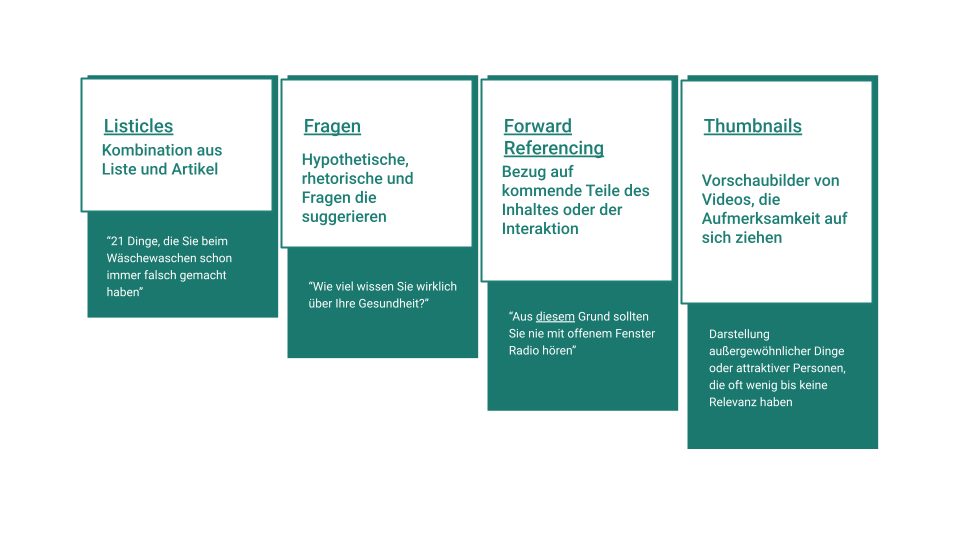
\includegraphics[width=14cm]{kapitel4/clickbaits.png}
    \caption[Die Kernformen des Clickbaits]{Die 4 Kernformen des Clickbaits in Anlehnung an \cite*[71]{Hrsg2020}}
    \label{TSNE}
\end{figure}

In \cite*[70-71]{Hrsg2020} werden CLickbaits formal in 4 Kategorien aufgeteilt. Der Autor bezieht sich dabei auf 4 Quellen und teilt Clickbaits als Listicles \cite*{Vijgen2014}, Fragen \cite*{Lai2014}, Forward Referencing \cite*{Blom2015} und Thumbnails \cite*{Zannettou2018} auf. Diese 4 Kategorien betrachtet der Autor als Kernkategorien. Aus \cite*[71]{Hrsg2020} werden Clickbaits außerdem in weitere Gestaltungsformen wie etwa, dass sie \enquote{Übertreibungen} sein können also falsche Versprechen geben, oder irreführend sind und unklar sein können.Es wird außerdem auf die unangemessene und vulgäre Sprache und der Formatierung, wie etwa den übertriebenen Gebrauch von Großschreibung oder Satzzeichen aufmerksam gemacht. Der Autor macht auf \cite*[75-76]{Hrsg2020} deutlich, dass Clickbaits kein neu eingesetztes Stilmittel im Journalismus sei. Schließlich verwendet der Autor den Begriff \enquote{Neugier} beim Leser. Leser wollen oftmals über Themen wie Tod, Gewalt, Sex und Prominente \cite*{Tenenboim2015} unterhalten werden.




\section{Wie werden Clickbaits klassifiziert?}
Mit der Arbeit aus \cite*{Chakrabortya} wurde eine Browser-Erweiterung erstellt, welches Clickbaits erkennen soll. Es wurden umfangreiche Daten sowohl für Clickbaits als auch für Nicht-Clickbait-Kategorien gesammelt. Für die Nicht-Clickbaits-Kategorien wurden 18.513 Wikinews Artikeln gesammelt. Der Vorteil dieser Artikel ist, dass diese von einer Community erstellt werden und jeder Nachrichtenartikel vor der Veröffentlichung von der Community geprüft werden. Es gibt Stilrichtlinien, die eingehalten werden müssen. Um Clickbaits zu finden, haben die Autoren manuell aus Seiten wie \enquote{Buzzfeed} oder \enquote{Upworthy} ca. 8000 Titel gecrawlt. Um falsche Negative zu vermeiden (d. h. die Artikel in diesen Bereichen, bei denen es sich nicht um Clickbaits handelt), wurden sechs Freiwillige rekrutiert um die Überschriften zu labeln. Schließlich wurden 7500 Titel zu jeder der beiden Kategorien zugefügt.

% \section{Analyse Textdaten}


Laut \cite*{Chakrabortya} sind die herkömmlichen Nicht-Clickbait Schlagzeilen kürzer als Clickbait Schlagzeilen. Traditionelle Schlagzeilen enthalten in der Regel meistens Wörter, die sich auf bestimmte Personen und Orte beziehen, während die Funktionswörter den Lesern zur Interpretation aus dem Kontext überlassen bleiben. Es wird hier als Beispiel gegeben \enquote{Visa-Deal oder kein Migranten-Deal, Türkei warnt EU}. Hier sind die meisten Wörter Inhaltswörter, die die wichtigsten Erkenntnisse aus der Geschichte zusammenfassen, und es gibt nur sehr wenige Verbindungsfunktionswörter zwischen den Inhaltswörtern. Auf der anderen Seite sind Clickbait Schlagzeilen länger. Die Sätze, enthalten sowohl Inhalts- als auch Funktionswörter. Ein Beispiel für solche Schlagzeilen ist \enquote{Ein 22-Jähriger, dessen Ehemann und Baby von einem betrunkenen Fahrer getötet wurden, hat ein Facebook-Plädoyer veröffentlicht}. Obwohl die Anzahl der Wörter in Clickbait-Schlagzeilen höher ist, ist die durchschnittliche Wortlänge kürzer. Es werden häufig Wörter verwendet wie \enquote{Sie werden}, \enquote{Sie sind}. Im Durchschnitt haben die Wörter bei den Clickbaits längere Abhängigkeiten als Nicht-Clickbaits. Der Hauptgrund ist die Existenz komplexerer Phrasensätze im Vergleich zu Schlagzeilen ohne Clickbait. Es ist außerdem zu sehen, dass in Clickbait-Schlagzeilen Stoppwörter häufiger verwendet werden. Clickbait Überschriften verwenden häufig Determinantien wie \enquote{ihre}, \enquote{meine}, die auf bestimmte Personen oder Dinge im Artikel verweisen. Die Verwendung Wörter dient in erster Linie dazu, den Benutzer neugierig auf das Objekt zu machen, auf das verwiesen wird, und ihn zu überzeugen, den Artikel weiter zu verfolgen. Um Daten zu erfassen, können auch Soziale Medien wie Twitter herangezogen werden, wie im Beispiel von \cite*{Potthast}.


% \section{Feature Selection}
Um lexikalischer und semantische und orthografische und morphologische Merkmale zu erfassen, benutzen die Autoren aus \cite*{Anand2019} Worteinbettungen und Zeicheneinbettungen, anstatt übermäßig Feature Selection auszuüben. Um Informationen außerhalb einzelner oder fester Wortfenster zu erfassen, untersuchten die Autoren dabei verschiedene RNN-Architekturen (Recurrent Neural Network) wie LSTM (Long Short Term Memory), GRU (Gated Recurrent Units) und Standard-RNNs. Dieses sind Wiederkehrende neuronale Netzwerkmodelle, die für sequentielle Daten wie Sprache und Text gut modelliert werden können.


Die Arbeit von \cite*{Agrawal2017} schlägt ein Modell vor, welches CNNs benutzt. CNNs werden für verschiedene Deep-Learning-Aufgaben verwendet. Es wurde nur eine Faltungsschicht in das CNN-Modell eingebaut. Die erste Schicht wird für das Einbetten der Wörter in Vektoren verwendet. Dabei wurden 2 verschiedene Worteinbettungen in Bezug genommen. Ein vortrainiertes und eines welches von Grund auf lernen musste und sich während des Trainings weiterentwickelt. In der nächsten Schicht werden Filter in verschiedenen Größen verwendet um Faltungen über Wortvektoren zu erzeugen.

Die Autoren der Arbeit aus \cite*{Pujahari} Clustern zunächst die aus den Schlagzeilen erstellten Vektoren mit der sogenannten t-SNE Methode nach \cite{VanDerMaaten2008}. Dieser Algorithmus \enquote{rekategorisiert} die Schlagzeilen in mehrere Gruppen und reduziert die vielen Dimensionen von Clickbaits im Datensatz. Die Autoren beginnen erst im nächsten Schritt mit dem Training. Dabei entstehen 11 Kategorien von Clickbaits (Mehrdeutig, Übertreibung oder Neckerei).


\begin{figure}[H]
    \centering
    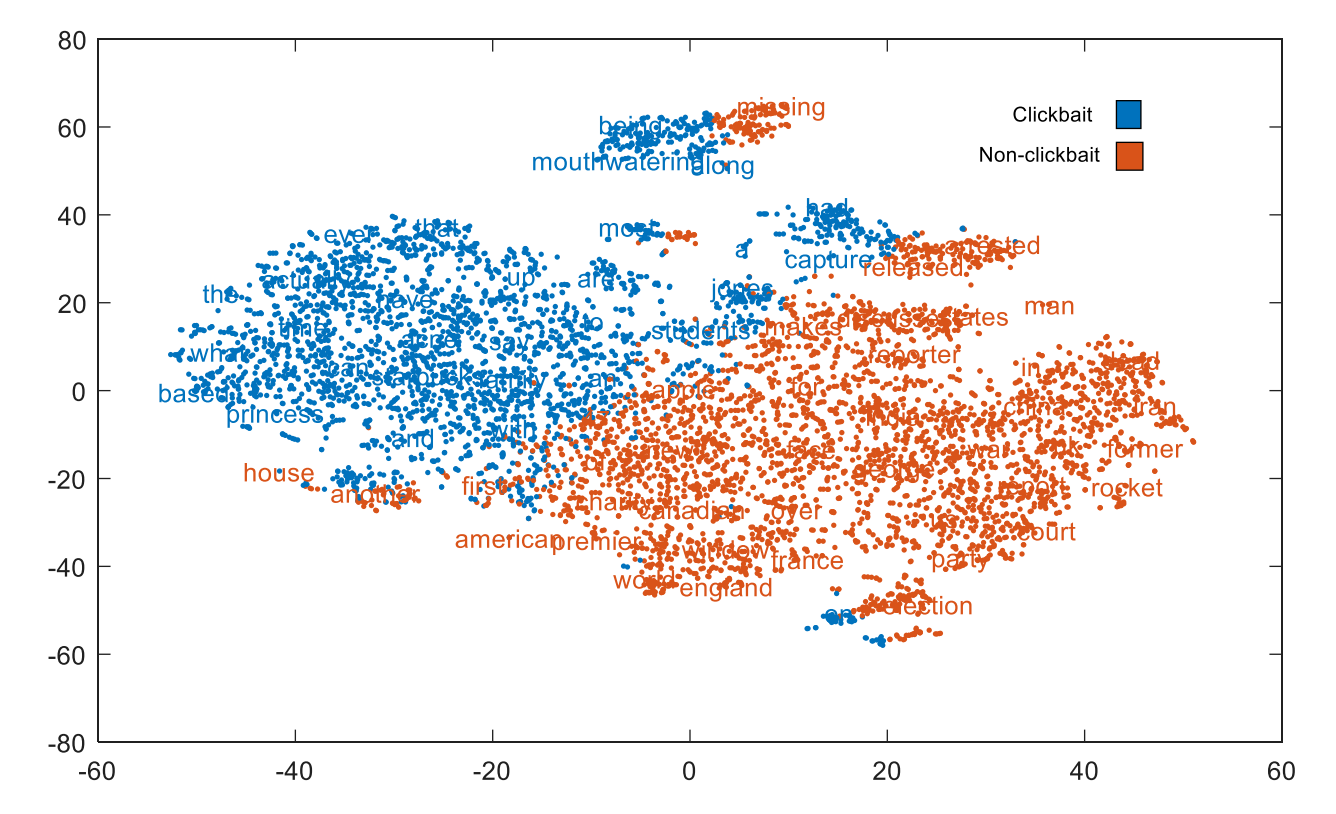
\includegraphics[width=12cm]{kapitel4/tsne.png}
    \caption[Clustering von Überschriften mit t-SNE]{Die Autoren verwenden das t-SNE Algorithmus nach \cite{VanDerMaaten2008} um die Dimensionen zu Reduzieren und es entstehen mehrere Unterkategorien von Clickbaits. Entnommen aus \cite*{Pujahari}.}
    \label{TSNE}
\end{figure}

\section{Schluss}
In diesem Kapitel wurden einige Arbeiten aus der Literatur vorgestellt, jedoch nicht alle. Es gibt außerdem noch weitere Arbeiten wie \cite*{chawda2019novel}\cite*{Zannettou2018}\cite*{Kumar}\cite*{Thomas}\cite*{Liao}\cite*{Glenski} und \cite*{Biyani2016} die unter diese Literaturstudie fallen könnten. Alle diese Arbeiten in Ihrer ganzen Fülle zu beschreiben würde den Rahmen dieser Arbeit sprengen, sodass nur ein Einblick über mögliche Aufgaben, wie das Sammeln von Daten und das Bauen eines Deep Learning Ansatzes sowie die Besonderheiten die Clickbaits Schlagzeilen haben, verschafft wurde.


% \section{Anwendung von Deep Learning Modellen}


% \label{Kap4}

% Die folgende Checkliste kann dazu dienen, die Arbeit auf die wichtigsten Bewertungskriterien zu prüfen. Jeder Dozent hat andere Kriterien, die unten aufgeführten dürften aber für die meisten Dozenten gültig sein.

% \section{Form und Sprache}

% \begin{checklist}
%   \footnotesize
%   \item \textbf{Aufbau}: Die Arbeit ist nach wissenschaftlichen Prinzipien aufgebaut (wesentliche Teile vorhanden, Nummerierung/Verweise korrekt, Verzeichnisse vorhanden).
%     \begin{checklist}
%         \item \textit{Wesentliche Teile}: Die folgenden Elemente der Arbeit sind vorhanden: Titelblatt, Abstract/Zusammenfassung, Einleitung, Hauptteil, Fazit/Ausblick.
%         \item \textit{Nummerierung/Verweise}: Das Nummerierungsschema wird konsistent über die gesamte Arbeit durchgehalten, die Verweise auf die verschiedenen Elemente (Abbildungen, Tabellen etc.) sind korrekt.
%         \item \textit{Verzeichnisse}: Die Arbeit enthält alle relevanten Verzeichnisse: Inhaltsverzeichnis, Literaturverzeichnis, Abbildungsverzeichnis, Tabellenverzeichnis, eventuell Glossar.
%     \end{checklist}
%   \item \textbf{Sprache}: Die verwendete Sprache entspricht wissenschaftlichen Ansprüchen.
%     \begin{checklist}
%         \item \textit{Begriffe und Definitionen}: Begriffe werden einheitlich und konsistent verwendet. Neue Begriffe werden definiert und mit Literatur hinterlegt.
%         \item \textit{Abkürzungen}: Alle Abkürzungen werden eingeführt und erläutert. Abkürzungen werden bei der ersten Verwendung ausgeschrieben und in einem Abkürzungsverzeichnis geführt. Es werden keine unüblichen oder selbst erfunden Abkürzungen verwendet. Ein Glossar kann verwendet werden, um Begriffe noch einmal kompakt darzustellen.
%         \item \textit{Rechtschreibung}: Die Arbeit ist frei von Rechtschreibungs-, Zeichensetzungs- und Grammatikfehlern.
%     \end{checklist}
%   \item \textbf{Formatierung, Typographie}: Die Formatierung der Arbeit ist korrekt und aus typographischer Sicht einwandfrei. \textit{Wenn Sie dieses Template korrekt verwenden, sollte dieser Punkt automatisch durch die Verwendung von \LaTeX \ erledigt sein.}
%     \begin{checklist}
%         \item \textit{Korrekte Typographie}: Schriftarten werden korrekt verwendet (nicht mehr als 2 Fonts), der Zeilenabstand ist passend, die Ränder sind ausreichend, der Satz ist korrekt.
%         \item \textit{Satz von Abbildungen, Tabellen etc.}: Abbildungen sind in der richtigen Auflösung dargestellt, die Tabellen sind korrekt gesetzt, mathematische Formeln und Symbole sind sauber dargestellt.
%     \end{checklist}
%   \item \textbf{Abbildungen}: Abbildungen werden in ausreichendem Umfang zur Förderung des Verständnisses eingesetzt. Sie werden korrekt im Text referenziert und sind, wo immer möglich, in einer Standardnotation erstellt.
%     \begin{checklist}
%         \item \textit{Ausreichende Verwendung}: Komplizierte Sachverhalte werden durch Abbildungen verdeutlicht. Es werden genug Abbildungen eingesetzt, um die wichtigsten Sachverhalte zu erklären.
%         \item \textit{Verständnisförderung}: Abbildungen dienen nicht als Schmuck, sondern um komplizierte Sachverhalte zu verdeutlichen.
%         \item \textit{Einbindung in den Text}: Der Text muss auch ohne Abbildungen verständlich sein, die Abbildungen helfen Sachverhalte aus dem Text besser darzustellen. Der Text referenziert die Abbildung korrekt.
%         \item \textit{Standardnotation, Legende}: Die Abbildungen verwenden Standard"=Notationen wie UML, FMC etc. Wo keine Standardnotation eingesetzt wird, ist eine Legende vorhanden, um die Bildelemente zu erläutern.
%     \end{checklist}
%   \item \textbf{Zitate}: Quellen werden konsistent nach einer gängigen Zitierweise zitiert und sind vollständig im Literaturverzeichnis angegeben.
%     \begin{checklist}
%         \item \textit{Zitierweise}: Die Zitierweise in der gesamten Arbeit folgt einem einheitlichen Schema, z.B. IEEE, DIN, Chicago.
%         \item \textit{Vollständigkeit}: Alle Zitate sind als solche kenntlich gemacht und die Quelle wird vollständig angegeben, und Plagiate werden vermieden.
%     \end{checklist}
%   \item \textbf{Schreibstil}: Lebendiger, wissenschaftlicher und verständlicher Schreibstil.
%     \begin{checklist}
%         \item \textit{Wissenschaftlichkeit}: Der Text ist im Präsenz geschrieben, es wird die dritte Person verwendet, Fachausdrücke werden korrekt verwendet, Fremdwörter und Amerikanismen werden richtig eingesetzt.
%         \item \textit{Verständlichkeit}: Abschweifungen und Wiederholungen werden vermieden, statt dessen werden präzise und übersichtliche Sätze verwendet.
%         \item \textit{Lebendigkeit}: Der Text der Arbeit zeichnet sich durch eine gute Wortwahl, Sprachbilder, einen angemessenen Satzbau und eine hohe Variabilität aus.
%     \end{checklist}
% \end{checklist}

% \section{Inhalt}

% \begin{checklist}
%   \footnotesize
%   \item \textbf{Gliederung}: Die Gliederung ist vollständig, konsistent und sachlogisch mit angemessener Struktur und Tiefe.
%     \begin{checklist}
%         \item \textit{Konsistenz und Vollständigkeit}: Auf einer Ebene stehen keine Punkte alleine, die Gliederungspunkte orientieren sich an der Argumentationskette.
%         \item \textit{Angemessene Tiefe}: Die Größe der einzelnen Unterpunkte ist vom Umfang her ähnlich. Es gibt keine Gliederungspunkte, die nur aus ein bis zwei Sätzen bestehen.
%     \end{checklist}
%   \item \textbf{Grundlagen}: Es werden alle relevanten Grundlagen gelegt. Der State"=of"=the"=art und der State"=of"=practice werden dargelegt.
%     \begin{checklist}
%         \item \textit{Umfang}: 1/3 des Hauptteils ist ein gutes Maß für eine ausreichende Darstellung der Grundlagen.
%         \item \textit{Begriffe und Methoden}: Begriffe und Methoden sind definiert, und Literatur zu den Definitionen ist angegeben.
%         \item \textit{State-of-the-art}: Der Stand des verfügbaren Wissens wird dargestellt, analysiert und kritisch beurteilt (state-of-the-art). Bei theoretischen Arbeiten kann ein eigenes Kapitel \enquote{verwandte Arbeiten} nötig sein, um den state"=of"=the"=art darzustellen.
%         \item \textit{State-of-practice}: Bei praktischen Arbeiten, die in der Industrie geschrieben werden, kann es nötig sein, auch das Vorgehen im Unternehmen zu erläutern.
%     \end{checklist}
%   \item \textbf{Methodik/Lösung}: Die gewählte Methodik bzw. Lösung ist für das Problem adäquat.
%     \begin{checklist}
%         \item \textit{Anforderungen an die Lösung}: Die von der Lösung zu erfüllenden Anforderungen werden dargestellt. Wo nötig wird dies auf Grundlage eines sauberen Requirements"=Engineerings durchgeführt.
%         \item \textit{Erläuterung des Lösungsansatzes}: Der gewählte Lösungsansatz wird ausführlich erläutert und verständlich dargestellt.
%         \item \textit{Eignung zur Lösung der Aufgabe}: Die gewählte Lösung ist geeignet, um das beschriebene Problem zu lösen.
%         \item \textit{Hypothesen}: Es sind ggf. Hypothesen gebildet worden; diese sind erläutert, und es sind Kriterien identifiziert worden, mit deren Hilfe man die Hypothesen falsifizieren kann.
%         \item \textit{Alternativen}: Es werden Alternativen zur vorgeschlagenen Lösung diskutiert. Die eigene Lösung wird nicht als einzige mögliche dargestellt, sondern es werden auch andere mögliche Lösungen vorgestellt und bewertet.
%         \item \textit{Begründung}: Alternativen und Kriterien für die Auswahl dieser Lösung werden dargestellt.
%         \item \textit{Vorteile der Lösung}: Es wird dargestellt, wieso die entwickelt Lösung vorteilhafter ist als die bisherigen Ansätze. Diese Darstellung erfolgt auf Basis des Lösungsansatzes. Eine konkrete Validierung der Implementierung erfolgt ggf. in späteren Kapiteln.
%     \end{checklist}
%   \item \textbf{Logik der Argumentationskette}: Die Argumentation ist logisch und nachvollziehbar. Sie ist frei von logischen Fehlschlüssen.
%   \item \textbf{Implementierung}: Wenn eine Implementierung der Lösung erfolgt, so wird die Implementierung beschrieben. Die Darstellung der Implementierung kann knapp ausfallen. Wichtig ist der Lösungsansatz, nicht die konkrete Umsetzung.
%   \item \textbf{Validierung}: Die vorgeschlagene Lösung wird ggf. empirisch verprobt.
%     \begin{checklist}
%         \item \textit{Vorgehensweise}: Die Vorgehensweise zur Validierung der Lösung / Hypothesen ist beschrieben und geeignet, relevante Aspekte der Lösung zu überprüfen.
%         \item \textit{Empirische Analyse}: Die Erfassungsmethode wird dargestellt und die Daten werden nach den Grundsätzen ordnungsgemäßer Laborpraxis gesammelt und statistisch korrekt ausgewertet.
%         \item \textit{Verprobung}: Die Lösung wird an einem praktischen Beispiel verprobt, und es werden wissenschaftlich korrekte Schlüsse aus der Anwendung gezogen.
%         \item \textit{Zielerreichung}: Funktioniert die gewählte Lösung nach der Implementierung? Wie weit wurde das Ziel erreicht? Falls nicht, gibt es nachvollziehbare Gründe dafür und wurden diese dargestellt?
%     \end{checklist}
%   \item \textbf{Diskussion}: Die Lösung und ihre Validierung wird kritisch und im Kontext möglicher Alternativen diskutiert und bewertet.
%     \begin{checklist}
%         \item \textit{Kritische Reflektion}: Grenzen und Schwächen der eigenen Ergebnisse werden beleuchtet.
%         \item \textit{Ableitung von Konsequenzen}: Die Konsequenzen aus den Ergebnissen für die Wissenschaft und Praxis sind beschrieben.
%     \end{checklist}
%   \item \textbf{Quellenarbeit}: Es werden hochwertige Quellen in ausreichendem Umfang genutzt und kritisch hinterfragt. Eventuell vorhandene Quellen aus dem Unternehmen werden ebenfalls berücksichtigt.
%     \begin{checklist}
%         \item \textit{Umfang}: Der Umfang an Quellen richtet sich stark nach Thema und Art der Arbeit. Bei einer Bachelorarbeit sind mindestens 20 Primärquellen und entsprechend viele Sekundärquellen üblich, bei einer Masterarbeit deutlich mehr.
%         \item \textit{Wissenschaftliche Qualität}: Nicht zitierfähig sind Internet"=Quellen, Wikipedia"=Einträge sowie andere Bachelor- oder Masterarbeiten (sofern nicht veröffentlicht). Das ausschließliche Zitieren von Lehrbüchern ist problematisch. Aktuelle wissenschaftliche Artikel und Werke sollten in den Quellen auftauchen.
%         \item \textit{Quellen \enquote{aus der Praxis}}: Wenn es im Unternehmen spezielle Quellen und Informationen gibt, so werden diese berücksichtigt, z. B. firmen- oder branchenspezifischer Informationen.
%         \item \textit{Kritische Würdigung}: Quellen und Zitate werden kritisch hinterfragt und nicht einfach unreflektiert übernommen. Es gibt eine kritische Distanz bei der Quellenauswahl und Quellenauswertung.
%     \end{checklist}
%   \item \textbf{Fazit}: Es wird eine Zusammenfassung der Arbeit sowie Ausblick auf weitere mögliche Arbeiten im Themenfeld gegeben, etwa die Lösung ausstehender Probleme oder die Erfüllung zusätzlicher Anforderungen.
%   \item \textbf{Umfang der Arbeit}: Richtgrößen: Bachelorarbeiten: 50--80 Seiten, Masterarbeiten: 60--100 Seiten, jeweils ohne Verzeichnisse und Anhang.
% \end{checklist}

% \section{Vor der Abgabe}

% \begin{checklist}
%   \footnotesize
%   \item \textit{Korrektur}: Haben Sie einen Dritten die Arbeit lesen lassen und alle gefundenen Rechtschreib- und Zeichensetzungsfehler behoben?
%   \item \textit{Literaturverzeichnis}: Sind im Literaturverzeichnis irrelevante Informationen entfernt? Beispielsweise bei Büchern unnötige Informationen über die Herkunft bei Google-Books oder bei Papern doppelte Angaben der DOI?
%   \item \textit{Doppel- oder einseitiger Druck}: Entspricht die Einstellung des Templates dem Druck, d.\,h. ist das Template für doppelseitigen Druck eingestellt, wenn doppelseitig gedruckt werden soll und umgekehrt?
%   \item \textit{Umschläge}: Sind die Umschläge vorhanden, um die Arbeit später zu binden? Die Umschläge können in der Hausdruckerei der Hochschule erworben werden.
%   \item \textit{Copyshop}: Wissen Sie, wo Sie die Arbeit drucken werden? Die Hausdruckerei kann Ihre Arbeit nicht drucken.
%   \item \textit{Exemplare}: Haben Sie geklärt, ob der Zweitkorrektor auch ein gedrucktes Exemplar möchte?
% \end{checklist}
